\section{矩阵分解}

\subsection{矩阵的三角分解}

矩阵的三角分解包括 LU 分解、LDU 分解、Doolittle 分解、Crout 分解和 Cholesky 分解等,其基本思想来自于\textbf{高斯消元法}。

\begin{definition}[初等矩阵]
初等行变换可以用左乘初等矩阵表示:
\begin{itemize}
    \item 交换两行:设 $u_{i,j}=(e_i-e_j)/\sqrt{2}$,
    \[
        I-2u_{i,j}u_{i,j}^T
    \]

    \item 第 $i$ 行乘以 $\alpha$ 加到第 $j$ 行:
    \[
        I+\alpha e_je_i^T
    \]

    \item 第 $i$ 行乘以 $\alpha$:
    \[
        I+(\alpha-1)e_ie_i^T
    \]
\end{itemize}
\end{definition}

\begin{definition}[消元因子]
第 $k$ 步消元时,若 $a_{kk}^{(k)}\neq 0$,则乘上消元因子 $m_{ik}=a_{ik}^{(k)}/a_{kk}^{(k)}$ 减到第 $i$ 行,其中 $i=k+1,\ldots,n$. 这相当于左乘矩阵: 
\[
    L_k=I-\left(\sum_{i=k+1}^nm_{ik}e_i\right)e_k^T=I-l_ke_k^T
\]
其中 $l_k=(0,\ldots,0,m_{k+1,k},m_{k+2,k},\ldots,m_{nk})^T$.
\end{definition}

\begin{theorem}
消元过程不改变矩阵的顺序主子式。
\end{theorem}

\begin{lemma}
约化的主元素 $a_{ii}^{(i)}\neq 0$ 的充要条件是矩阵 $A$ 的顺序主子式 $D_i\neq 0\,(i=1,\ldots,k)$.
\end{lemma}

\begin{corollary}
若矩阵 $A$ 的顺序主子式 $D_i\neq 0\,(i=1,\ldots,k)$,则:
\[
    a_{11}^{(1)}=D_1,\quad a_{ii}^{(i)}=D_i/D_{i-1}
\]
\end{corollary}

\begin{theorem}
若 $A$ 是正定矩阵,则一次消元后剩下的矩阵依旧是正定的。
\end{theorem}

\begin{theorem}
若 $A$ 严格对角占优,则一次消元后剩下的矩阵依旧是严格对角占优的。
\end{theorem}

\begin{definition}[LU 分解]
若方阵 $A$ 可以分解为一个下三角矩阵 $L$ 和一个上三角矩阵 $U$ 的乘积,即 $A=LU$,则称 $A$ 可作 LU 分解。
\end{definition}

\begin{com}
高斯消元的过程可以用 LU 分解表示:
\[
    \underbrace{L_{n-1}L_{n-2}\cdots L_2L_1}_{L^{-1}} A=U\implies A=LU
\]
其中 $L$ 为\textbf{单位}下三角矩阵,$U$ 为上三角矩阵。
\end{com}

\begin{definition}[LDU 分解]
若方阵 $A$ 可分解为 $A=LDU$,其中 $L$ 为\textbf{单位}下三角矩阵,$U$ 为\textbf{单位}上三角矩阵,$D$ 为对角矩阵,则称 $A$ 可作 LDU 分解。
\end{definition}

\begin{theorem}
设 $A$ 是 $n$ 阶方阵,当且仅当 $A$ 的顺序主子式 $\Delta_i\neq 0$ 时,$A$ 可唯一分解为 $A=LDU$,其中:
\[
    D=\text{diag}(d_1,\ldots,d_n),\quad d_k=\frac{\Delta_k}{\Delta_{k-1}}
\]
\end{theorem}

\begin{corollary}
$n$ 阶非奇异方阵 $A$ 有 LU 分解 $A=LU$ 的充要条件是顺序主子式 $\Delta_i\neq 0$.
\end{corollary}

\begin{theorem}
设 $A$ 是 $n$ 阶非奇异矩阵,则存在置换矩阵 $P$ 使得 $PA$ 的 $n$ 个顺序主子式非零。
\end{theorem}

\begin{corollary}[带有置换矩阵的三角分解]
设 $A$ 是 $n$ 阶非奇异方阵,则存在置换矩阵 $P$,使得:
\[
    PA=L\hat U=LDU
\]
其中 $L$ 为\textbf{单位}下三角矩阵,$\hat U$ 为上三角矩阵,$U$ 为\textbf{单位}上三角矩阵,$D$ 为对角矩阵。
\end{corollary}


\begin{definition}[Doolittle 分解]
把 LDU 分解中的 $DU$ 结合起来用 $\hat U$ 表示,得到唯一的分解:
\[
    A=L(DU)=L\hat U
\]
\end{definition}
\begin{definition}[Crout 分解]
把 LDU 分解中的 $LD$ 结合起来用 $\hat L$ 表示,得到唯一的分解:
\[
    A=(LD)U=\hat LU
\]
\end{definition}

\noindent\textbf{计算方法(以 Doolittle 分解为例)}:比较等式两边的元素逐行逐列求解 $L,U$ 各元素:
\[
    \begin{bmatrix}
    a_{11}&a_{12}&\cdots&a_{1n}\\
    a_{21}&a_{22}&\cdots&a_{2n}\\
    \vdots&\vdots&\ddots&\vdots\\
    a_{n1}&a_{n2}&\cdots&a_{nn}\\
    \end{bmatrix}=
    \begin{bmatrix}
    1&&&\\
    l_{21}&1&&\\
    \vdots&\vdots&\ddots&\\
    l_{n1}&l_{n2}&\cdots&1\\
    \end{bmatrix}
    \begin{bmatrix}
    u_{11}&u_{12}&\cdots&u_{1n}\\
    &u_{22}&\cdots&u_{2n}\\
    &&\ddots&\vdots\\
    &&&u_{nn}\\
    \end{bmatrix}
\]
\begin{figure}[H]
    \centering
    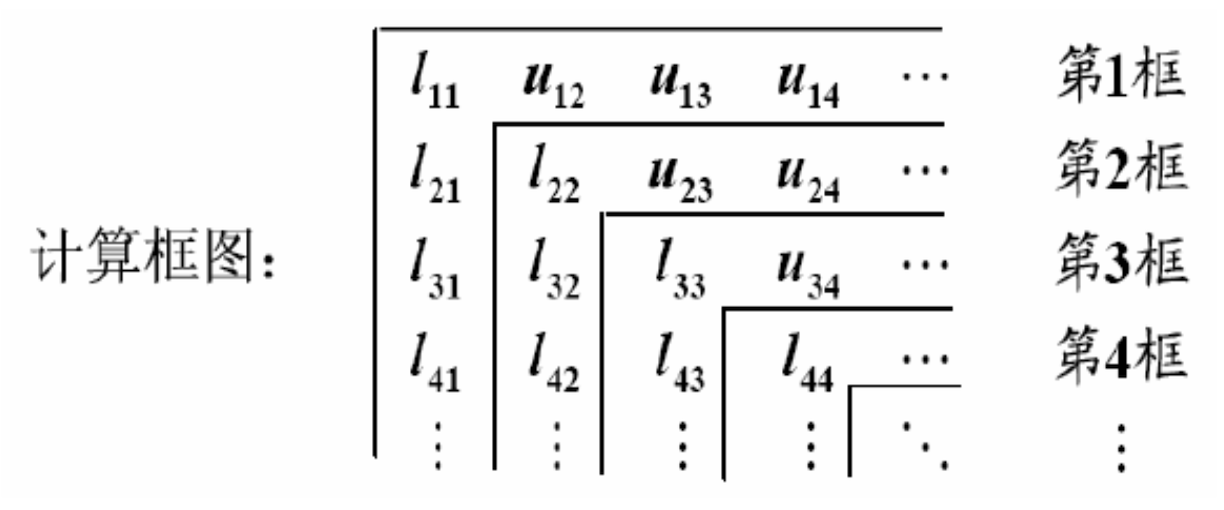
\includegraphics[width=0.5\linewidth]{figs/calc.png}
\end{figure}

\begin{definition}[Cholesky 分解]
若实对称正定矩阵可以按如下方式分解:
\[
    A=L\tilde D^2L^T\quad\text{或}\quad A=LDL^T\quad\text{或}\quad A=LL^T
\]
则称 $A$ 可作 Cholesky 分解。其中第二种表示中,$D$ 的对角元都大于零;第三种表示中,$L$ 的对角元都大于零。
\end{definition}

\noindent\textbf{计算方法}:与 Doolittle 分解的计算类似,逐行逐列计算即可:
\[
    \begin{bmatrix}
    a_{11}&a_{12}&\cdots&a_{1n}\\
    a_{21}&a_{22}&\cdots&a_{2n}\\
    \vdots&\vdots&\ddots&\vdots\\
    a_{n1}&a_{n2}&\cdots&a_{nn}\\
    \end{bmatrix}=
    \begin{bmatrix}
    l_{11}&&&\\
    l_{21}&l_{22}&&\\
    \vdots&\vdots&\ddots&\\
    l_{n1}&l_{n2}&\cdots&l_{nn}\\
    \end{bmatrix}
    \begin{bmatrix}
    l_{11}&l_{12}&\cdots&l_{1n}\\
    &l_{22}&\cdots&l_{2n}\\
    &&\ddots&\vdots\\
    &&&l_{nn}\\
\end{bmatrix}
\]
可得:
\[
    l_{jj}=\left(a_{jj}-\sum_{k=1}^{j-1}l_{jk}^2\right)^{1/2},\quad l_{ij}=\left(a_{ij}-\sum_{k=1}^{j-1}l_{ik}l_{jk}\right)/l_{jj}
\]
该计算方法的缺点是有开方运算,在计算机中由于浮点误差可能出现根号下负数。

\vskip 10pt \noindent\textbf{改进的 Cholesky 分解计算方法}:所谓改进的 Cholesky 分解,其实就是指 $A=LDL^T$,其计算过程不涉及开方,因而有更好的数值稳定性:
\[
    \begin{bmatrix}
    a_{11}&a_{12}&\cdots&a_{1n}\\
    a_{21}&a_{22}&\cdots&a_{2n}\\
    \vdots&\vdots&\ddots&\vdots\\
    a_{n1}&a_{n2}&\cdots&a_{nn}\\
    \end{bmatrix}=
    \begin{bmatrix}
    1&&&\\
    l_{21}&1&&\\
    \vdots&\vdots&\ddots&\\
    l_{n1}&l_{n2}&\cdots&1\\
    \end{bmatrix}
    \begin{bmatrix}
    d_1&d_1l_{12}&\cdots&d_1l_{1n}\\
    &d_2&\cdots&d_2l_{2n}\\
    &&\ddots&\vdots\\
    &&&d_n\\
    \end{bmatrix}
\]
逐行逐列计算可得:
\[
    l_{ij}=\left(a_{ij}-\sum_{k=1}^{j-1}l_{ik}d_kl_{jk}\right)/d_j,\quad d_i=a_{ii}-\sum_{k=1}^{j-1}l_{ik}^2d_k
\]

\begin{definition}[分块矩阵的拟 LU 分解和拟 LDU 分解]
只考虑 2 阶的分块矩阵:
\[
    A=\begin{bmatrix}A_{11}&A_{12}\\A_{21}&A_{22}\end{bmatrix}
\]
若 $A_{11}$ 可逆,设:
\[
    L=\begin{bmatrix}I_{n_1}&0\\-A_{21}A_{11}^{-1}&I_{n_2}\end{bmatrix}
\]
则:
\[
    LA=\begin{bmatrix}A_{11}&A_{12}\\0&A_{22}-A_{21}A_{11}^{-1}A_{12}\end{bmatrix}
\]
若 $A_{22}$ 可逆,可右乘矩阵(作列变换)得到类似的结果。
\end{definition}

\begin{lemma}[求逆引理 / Woodbury 公式]
\[
    (A+BC)^{-1}=A^{-1}-A^{-1}B(I+CA^{-1}B)^{-1}CA^{-1}
\]
\end{lemma}
\begin{proof}
考虑方程 $(A+BC)x=b$,令 $y=Cx$,则:
\[
    \begin{bmatrix}A&B\\-C&0\end{bmatrix}\begin{bmatrix}x\\y\end{bmatrix}=\begin{bmatrix}b\\0\end{bmatrix}
\]
利用高斯消元法:
\begin{figure}[H]
    \centering
    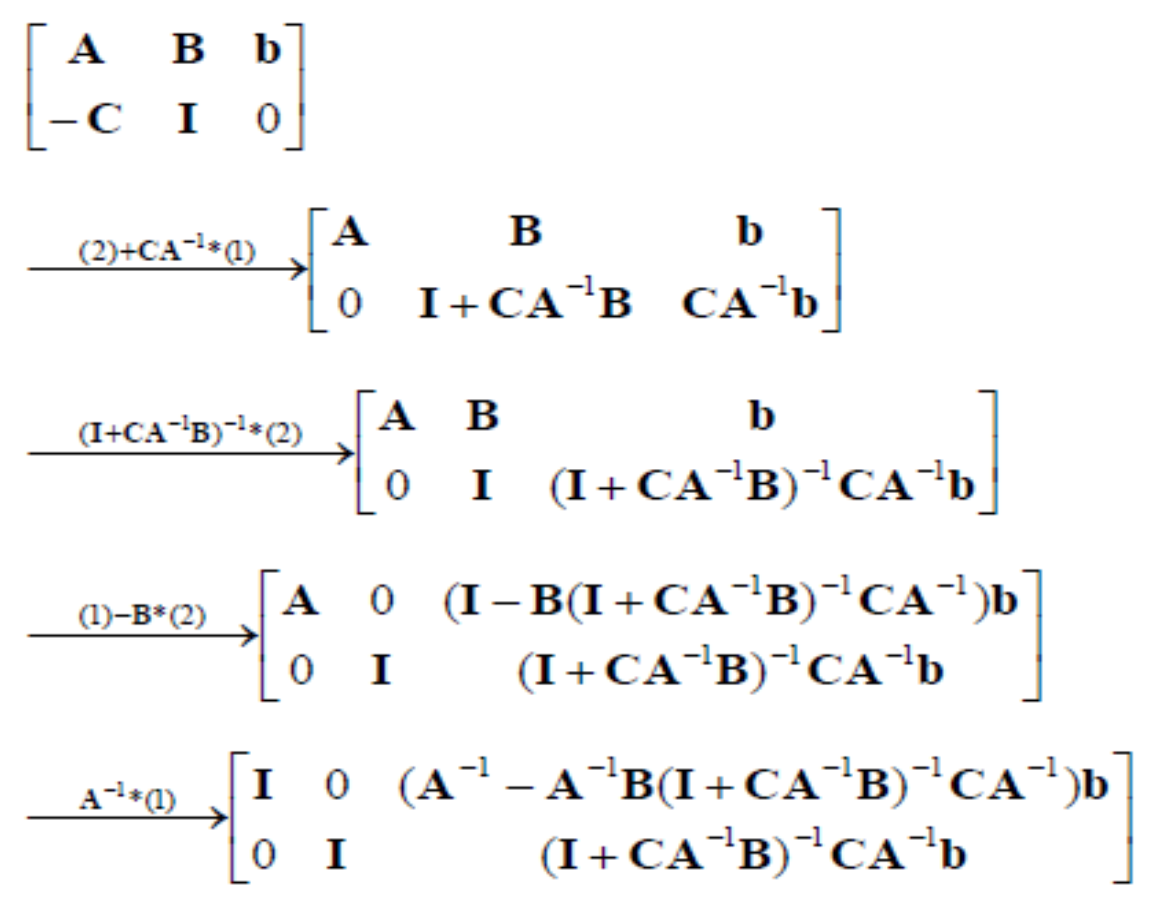
\includegraphics[width=0.5\linewidth]{figs/gauss.png}
\end{figure}
故解得:
\[
    x=(A^{-1}-A^{-1}B(I+CA^{-1}B)^{-1}CA^{-1})b
\]
又 $x=(A+BC)^{-1}b$,由 $b$ 的任意性可知命题成立。
\end{proof}

\begin{corollary}
\[
    (A+BD^{-1}C)^{-1}=A^{-1}-A^{-1}B(D+CA^{-1}B)^{-1}CA^{-1}
\]
\end{corollary}


\subsection{矩阵的 QR 分解}
\label{sec:qr}

\begin{definition}[Givens 矩阵,Givens 变换]
设 $c,s\in\mathbb R$ 且 $c^2+s^2=1$,称:
\[
    T_{ij}=T_{ij}(c,s)=
    \begin{bmatrix}
    1&      & &  & &      & & & &      & \\
     &\ddots& &  & &      & & & &      & \\
     &      &1&  & &      & & & &      & \\
     &      & &c & &      & &s& &      & \\
     &      & &  &1&      & & & &      & \\
     &      & &  & &\ddots& & & &      & \\
     &      & &  & &      &1& & &      & \\
     &      & &-s& &      & &c& &      & \\
     &      & &  & &      & & &1&      & \\
     &      & &  & &      & & & &\ddots& \\
     &      & &  & &      & & & &      &1\\
    \end{bmatrix}
\]
为 Givens 矩阵。由 Givens 矩阵确定的线性变换称作 Givens 变换(初等旋转变换)。
\end{definition}

\begin{remark}
顾名思义,Givens 变换的作用是旋转。具体而言,是在第 $i$ 和第 $j$ 维的平面上绕原点\textbf{顺时针}旋转 $\theta$,其中 $c=\cos\theta,\,s=\sin\theta$.
\end{remark}

\begin{property}
Givens 矩阵是正交矩阵,且有:
\[
    [T_{ij}(c,s)]^{-1}=[T_{ij}(c,s)]^T=T_{ij}(c,-s),\quad\det(T_{ij}(c,s))=1
\]
\end{property}

\begin{theorem}
设 $x=(\xi_1,\ldots,\xi_n)^T\neq0$,则存在有限个 Givens 矩阵的乘积,记作 $T$,使得 $Tx=|x|e_1$.
\end{theorem}
\begin{proof}[证明(构造性)]
构造 Givens 矩阵 $T_{12}(c,s)$:
\[
    c=\frac{\xi_1}{\sqrt{\xi_1^2+\xi_2^2}}\quad s=\frac{\xi_2}{\sqrt{\xi_1^2+\xi_2^2}}
\]
则:
\[
    T_{12}x=\left(\sqrt{\xi_1^2+\xi_2^2},0,\xi_3,\ldots,\xi_n\right)^T
\]
再对 $T_{12}x$ 构造 Givens 矩阵 $T_{13}(c,s)$:
\[
    c=\frac{\sqrt{\xi_1^2+\xi_2^2}}{\sqrt{\xi_1^2+\xi_2^2+\xi_3^2}}\quad s=\frac{\xi_3}{\sqrt{\xi_1^2+\xi_2^2+\xi_3^2}}
\]
则:
\[
    T_{13}(T_{12}x)=\left(\sqrt{\xi_1^2+\xi_2^2+\xi_3^2},0,0,\xi_4,\ldots,\xi_n\right)^T
\]
如此继续下去,最后对 $T_{1,n-1}\cdots T_{12}x$ 构造 Givens 矩阵 $T_{1n}(c,s)$:
\[
    c=\frac{\sqrt{\xi_1^2+\cdots\xi_{n-1}^2}}{\sqrt{\xi_1^2+\cdots\xi_{n-1}^2+\xi_n^2}}\quad s=\frac{\xi_n}{\sqrt{\xi_1^2+\cdots\xi_{n-1}^2+\xi_n^2}}
\]
则:
\[
    T_{1n}(T_{1,n-1}\cdots T_{12}x)=\left(\sqrt{\xi_1^2+\cdots\xi_n^2},0,\ldots,0\right)^T
\]
令 $T=T_{1n}T_{1,n-1}\cdots T_{12}$,则 $Tx=|x|e_1$.
\end{proof}
\begin{remark}
直观理解:依次把第 $2,3,\ldots,n$ 维转到 0 即可。
\end{remark}

\begin{corollary}
任给非零列向量 $x\in\mathbb R^n$ 及单位列向量 $z\in\mathbb R^n$,则存在有限个 Givens 矩阵的乘积,记作 $T$,使得 $Tx=|x|z$.
\end{corollary}

\noindent\textbf{快速 Givens 变换}:暂略。

\begin{definition}[Householder 矩阵,Householder 变换]
设 $u\in\mathbb R^n$ 是单位列向量,称:
\[
    H=I-2uu^T
\]
为 Householder 矩阵。由 Householder 矩阵确定的线性变换称作 Householder 变换(初等反射变换)。
\end{definition}

\begin{remark}
顾名思义,Householder 变换的作用是反射。具体而言,是对以 $u$ 为法向量的平面做反射。
\end{remark}

\begin{property}
Householder 矩阵对称、正交、对合、自逆,且行列式为 $-1$:
\[
    H^T=H,\quad H^TH=I,\quad H^2=I,\quad H^{-1}=H,\quad \det(H)=-1
\]
\end{property}

\begin{theorem}
任给非零列向量 $x\in\mathbb R^n$ 及单位列向量 $z\in\mathbb R^n$,则存在 Householder 矩阵 $H$,使得 $Hx=|x|z$.
\end{theorem}
\begin{proof}[证明(构造性)]
若 $x=|x|z$,取单位向量 $u$ 使得 $u\perp x$,则 $H_u=I-2uu^T$:
\[
    H_ux=(I-2uu^T)x=x-2uu^Tx=x=|x|z
\]
否则,$x\neq|x|z$,取 $u=\dfrac{x-|x|z}{\left|x-|x|z\right|}$,则:
\begin{align*}
H_ux&=\left[I-2\frac{(x-|x|z)(x-|x|z)^T}{|x-|x|z|^2}\right]x\\
&=x-\frac{2(x-|x|z)^Tx}{|x-|x|z|^2}(x-|x|z)\\
&=x-(x-|x|z)=|x|z
\end{align*}
\end{proof}
\begin{remark}
直观理解:找到 $x$ 和 $z$ 之间对称平面,取 $u$ 为该平面的单位法向量即可。
\end{remark}

\begin{theorem}
Givens 变换可写作两个 Householder 变换的乘积。
\end{theorem}
\begin{remark}
换句话说,一次旋转操作可以分解为两次反射操作。
\end{remark}
\begin{proof}
取
\begin{align*}
    &u=(0,\ldots,0,\sin(\theta/4),0,\ldots,0,\cos(\theta/4),0,\ldots,0)^T\\
    &v=(0,\ldots,0,\sin(3\theta/4),0,\ldots,0,\cos(3\theta/4),0,\ldots,0)^T
\end{align*}
可以验证 $T_{ij}=H_vH_u$.
\end{proof}
\begin{note}
Householder 矩阵并不能由若干个 Givens 矩阵的乘积表示,因为 $\det(H)=-1$ 而 $\det(G)=1$.
\end{note}

\begin{definition}[QR 分解]
\label{def:qr}
若实/复矩阵 $A$ 能分解成正交/酉矩阵 $Q$ 与\textbf{非奇异}上三角矩阵 $R$ 的乘积,即 $A=QR$,则称 $A$ 可作 QR 分解。
\end{definition}

\begin{theorem}[非奇异方阵的 QR 分解]
\label{thm:qr1}
对 $n$ 阶\textbf{非奇异}矩阵 $A$,QR 分解在除去相差一个对角元素的绝对值/模全等于 1 的对角矩阵外,分解唯一。
\end{theorem}
\begin{proof}[证明(实数情形)]
设 $A=Q_1R_1=Q_2R_2$,则 $P=Q_2^TQ_1=R_2R_1^{-1}$. 注意到 $P^TP=I$,所以 $P^T=P^{-1}$.  由于 $P$ 是上三角矩阵,所以 $P^{-1}$ 是上三角矩阵,$P^T$ 是下三角矩阵,二者又相等,因此只能是对角矩阵。又 $P^2=I$,所以对角元只能是 $\pm1$.  那么 $Q_1=Q_2P,\,R_1=PR_2$.
\end{proof}

\begin{theorem}[列满秩矩阵的 QR 分解]
\label{thm:qr2}
对 $m\times n$ 实/复矩阵 $A$,其 $n$ 列线性无关(即 $A$ 列满秩),则 $A$ 有分解 $A=QR$,其中 $Q$ 是 $m\times n$ 实/复矩阵,且 $Q^HQ=I$(即 $Q$ 是正交/酉矩阵的一部分),$R$ 是实/复非奇异上三角矩阵,且除去相差一个对角元素的绝对值/模全等于 1 的对角矩阵外,分解唯一。
\end{theorem}

\noindent\textbf{计算方法(基于 Gram-Schmidt 正交化过程)}:
设 $A=(a_1,\ldots,a_n)$ 非奇异,对其各列实施 Gram-Schmidt 正交化过程:
\[
    \begin{cases}
    b_1=a_1\\
    b_2=a_2-k_{21}b_1\\
    \quad\vdots\\
    b_n=a_n-k_{n,n-1}b_{n-1}-\cdots-k_{n1}b_1
    \end{cases}\implies
    \begin{cases}
    a_1=b_1\\
    a_2=b_2+k_{21}b_1\\
    \quad\vdots\\
    a_n=b_n+k_{n,n-1}b_{n-1}+\cdots+k_{n1}b_1
    \end{cases}
\]
写作矩阵形式:
\begin{align*}
    A=BK&\implies(a_1,a_2,\ldots,a_n)=(b_1,b_2,\ldots,b_n)\begin{bmatrix}1&k_{21}&\cdots&k_{n1}\\&1&\cdots&k_{n2}\\&&\ddots&\vdots\\&&&1\end{bmatrix}\\
    &\implies(a_1,a_2,\ldots,a_n)=\underbrace{\begin{bmatrix}\dfrac{b_1}{|b_1|},\dfrac{b_2}{|b_2|}\ldots,\dfrac{b_n}{|b_n|}\end{bmatrix}}_Q\underbrace{\begin{bmatrix}|b_1|&&&\\&|b_2|&&\\&&\ddots&\\&&&|b_n|\end{bmatrix}\begin{bmatrix}1&k_{21}&\cdots&k_{n1}\\&1&\cdots&k_{n2}\\&&\ddots&\vdots\\&&&1\end{bmatrix}}_R\\
    &\implies A=QR
\end{align*}
\begin{note}
基于 Gram-Schmidt 正交化过程的 QR 分解计算方法在高阶时容易出现数值不稳定,需要用下文的基于 Givens 变换或 Householder 变换的方法计算。
\end{note}

\noindent\textbf{计算方法(基于 Givens 变换)}:
任何 $n$ 阶\textbf{实非奇异}矩阵 $A$ 都可以通过左连乘 Givens 初等旋转矩阵化为上三角矩阵。
\begin{enumerate}
    \item 由于 $\det(A)\neq0$,因此 $A$ 的第一列 $(a_{11},a_{21},\ldots,a_{n1})^T\neq 0$,根据前文的定理,存在有限个 Givens 矩阵的乘积 $T_1$,使得
    \[
        T_1(a_{11},a_{21},\ldots,a_{n1})^T=\left|(a_{11},a_{21},\ldots,a_{n1})^T\right|\cdot e_1
    \]
    将 $T_1$ 作用在 $A$ 上得:
    \[
        T_1A=\left[\begin{array}{c:ccc}
        a_{11}^{(1)}&a_{12}^{(1)}&\cdots&a_{1n}^{(1)}\\
        \hdashline
        0&&&\\
        \vdots&&A^{(1)}&\\
        0&&&
        \end{array}\right]
    \]

    \item 由于 $\det(A^{(1)})\neq0$,因此 $A^{(1)}$ 的第一列 $\left(a_{22}^{(1)},a_{32}^{(1)},\ldots,a_{n2}^{(1)}\right)^T\neq0$,于是存在有限个 Givens 矩阵的乘积 $T_2$,使得
    \[
        T_2\left(a_{22}^{(1)},a_{32}^{(1)},\ldots,a_{n2}^{(1)}\right)^T=\left|\left(a_{22}^{(1)},a_{32}^{(1)},\ldots,a_{n2}^{(1)}\right)^T\right|\cdot e_1
    \]
    将 $T_2$ 作用在 $A$ 上得:
    \[
        T_2A^{(1)}=\left[\begin{array}{c:ccc}
        a_{22}^{(2)}&a_{23}^{(2)}&\cdots&a_{2n}^{(2)}\\
        \hdashline
        0&&&\\
        \vdots&&A^{(2)}&\\
        0&&&
        \end{array}\right]
    \]

    \item 重复上述步骤,直到第 $n-1$ 步:
    \[
        T_{n-1}A^{(n-2)}=\begin{bmatrix}a_{n-1,n-1}^{(n-1)}&a_{n-1,n}^{(n-1)}\\0&a_{nn}^{(n- 1)}\end{bmatrix}
    \]

    \item 最后,令:
    \[
        T=\begin{bmatrix}I_{n-2}&O\\O&T_{n-1}\end{bmatrix}\cdots\begin{bmatrix}I_{2}&O\\O&T_{3}\end{bmatrix}\begin{bmatrix}I_{1}&O\\O&T_{2}\end{bmatrix}T_1
    \]
    则:
    \[
        TA=\begin{bmatrix}
        a_{11}^{(1)}&a_{12}^{(1)}&\cdots&a_{1,n-1}^{(1)}&a_{1n}^{(1)}\\
        &a_{22}^{(2)}&\cdots&a_{2,n-1}^{(2)}&a_{2n}^{(2)}\\
        &&\ddots&\vdots&\vdots\\
        &&&a_{n-1,n-1}^{(n-1)}&a_{n-1,n}^{(n-1)}\\
        &&&&a_{nn}^{(n-1)}
        \end{bmatrix}
    \]
    即 $A=QR$,其中 $Q=T^{-1}=T^T$,$R$ 就是上面化出来的那一大坨上三角矩阵。
\end{enumerate}

\begin{remark}
该过程与高斯消元法有异曲同工之妙。
\end{remark}

\noindent\textbf{计算方法(基于 Householder 变换)}:任何 $n$ 阶\textbf{实非奇异}矩阵 $A$ 都可以通过左连乘 Householder 初等反射矩阵化为上三角矩阵。
\begin{enumerate}
    \item 由于 $\det(A)\neq0$,因此 $A$ 的第一列 $(a_{11},a_{21},\ldots,a_{n1})^T\neq 0$,根据前文的定理,存在一个 Householder 矩阵 $H_1$,使得
    \[
        H_1(a_{11},a_{21},\ldots,a_{n1})^T=\left|(a_{11},a_{21},\ldots,a_{n1})^T\right|\cdot e_1
    \]
    将 $H_1$ 作用在 $A$ 上得:
    \[
        H_1A=\left[\begin{array}{c:ccc}
        a_{11}^{(1)}&a_{12}^{(1)}&\cdots&a_{1n}^{(1)}\\
        \hdashline
        0&&&\\
        \vdots&&A^{(1)}&\\
        0&&&
        \end{array}\right]
    \]
    
    \item 由于 $\det(A^{(1)})\neq0$,因此 $A^{(1)}$ 的第一列 $\left(a_{22}^{(1)},a_{32}^{(1)},\ldots,a_{n2}^{(1)}\right)^T\neq0$,于是存在一个 Householder 矩阵 $H_2$,使得
    \[
        H_2\left(a_{22}^{(1)},a_{32}^{(1)},\ldots,a_{n2}^{(1)}\right)^T=\left|\left(a_{22}^{(1)},a_{32}^{(1)},\ldots,a_{n2}^{(1)}\right)^T\right|\cdot e_1
    \]
    将 $H_2$ 作用在 $A$ 上得:
    \[
        H_2A^{(1)}=\left[\begin{array}{c:ccc}
        a_{22}^{(2)}&a_{23}^{(2)}&\cdots&a_{2n}^{(2)}\\
        \hdashline
        0&&&\\
        \vdots&&A^{(2)}&\\
        0&&&
        \end{array}\right]
    \]
   
    \item 重复上述步骤,直到第 $n-1$ 步:
    \[
        H_{n-1}A^{(n-2)}=\begin{bmatrix}a_{n-1,n-1}^{(n-1)}&a_{n-1,n}^{(n-1)}\\0&a_{nn}^{(n-1)}\end{bmatrix}
    \]

    \item 最后,令:
    \[
        H=\begin{bmatrix}I_{n-2}&O\\O&H_{n-1}\end{bmatrix}\cdots\begin{bmatrix}I_{2}&O\\O&H_{3}\end{bmatrix}\begin{bmatrix}I_{1}&O\\O&H_{2}\end{bmatrix}H_1
    \]
    则:
    \[
        HA=\begin{bmatrix}
        a_{11}^{(1)}&a_{12}^{(1)}&\cdots&a_{1,n-1}^{(1)}&a_{1n}^{(1)}\\
        &a_{22}^{(2)}&\cdots&a_{2,n-1}^{(2)}&a_{2n}^{(2)}\\
        &&\ddots&\vdots&\vdots\\
        &&&a_{n-1,n-1}^{(n-1)}&a_{n-1,n}^{(n-1)}\\
        &&&&a_{nn}^{(n-1)}
        \end{bmatrix}
    \]
    即 $A=QR$,其中 $Q=H^{-1}=H^T$,$R$ 就是上面化出来的那一大坨上三角矩阵。
\end{enumerate}

% ## Hessenberg 矩阵的正交相似

\begin{definition}[Hessenberg 矩阵]
称次对角线以下全为零的矩阵为 Hessenberg 矩阵。
\[
    F=\begin{bmatrix}
    a_{11}&a_{12}&a_{13}&\cdots&a_{1,n-1}&a_{1n}\\
    a_{21}&a_{22}&a_{23}&\cdots&a_{2,n-1}&a_{2n}\\
    0&a_{32}&a_{33}&\cdots&a_{3,n-1}&a_{3n}\\
    \vdots&\vdots&\vdots&\ddots&\vdots&\vdots\\
    0&0&0&\cdots&a_{n-1,n-1}&a_{n-1,n}\\
    0&0&0&\cdots&a_{n,n-1}&a_{nn}
    \end{bmatrix}
\]
\end{definition}

\begin{theorem}
\label{thm:hessenberg}
任何\textbf{实方阵}都可以通过初等旋转变换正交相似于 Hessenberg 矩阵。即:设 $A\in\mathbb R^{n\times n}$,则存在有限个 Givens 矩阵之积 $Q$,使得 $QAQ^T=F$.
\end{theorem}
\begin{proof}
\begin{enumerate}
    \item 对 $A$,若 $\beta^{(0)}=(a_{21},\ldots,a_{n2})^T\neq0$,则存在有限个 Givens 矩阵之积 $T_0$,使得 $T_0\beta^{(0)}=|\beta^{(0)}|e_1=a_{21}^{(1)}e_1$:
    \[
    \begin{bmatrix}1&\\&T_0\end{bmatrix}A\begin{bmatrix}1&\\&T_0\end{bmatrix}^T=
    \left[\begin{array}{c:cccc}
    a_{11}&a_{12}^{(1)}&a_{13}^{(1)}&\cdots&a_{1n}^{(1)}\\
    \hdashline a_{21}^{(1)}&&&&\\
    0&&&&\\
    \vdots&&&A^{(1)}&\\
    0&&&&
    \end{array}\right]
    \]
    若 $\beta^{(0)}=0$,转 2;

    \item 对 $A^{(1)}$,若 $\beta^{(1)}=(a_{32}^{(1)},\ldots,a_{n2}^{(1)})^T\neq0$,则存在有限个 Givens 矩阵之积 $T_1$,使得 $T_1\beta^{(1)}=|\beta^{(1)}|e_1=a_{32}^{(1)}e_1$:
    \[
        \begin{bmatrix}1&\\&T_1\end{bmatrix}A^{(1)}\begin{bmatrix}1&\\&T_1\end{bmatrix}^T=
        \left[\begin{array}{c:cccc}
        a_{22}&a_{23}^{(1)}&a_{24}^{(1)}&\cdots&a_{2n}^{(1)}\\
        \hdashline a_{32}^{(1)}&&&&\\
        0&&&&\\
        \vdots&&&A^{(2)}&\\
        0&&&&
        \end{array}\right]
    \]
    若 $\beta^{(1)}=0$,转 3;

    \item 反复执行上述操作,直到 $n-2$ 步结束。

    \item 最后,令:
    \[
        Q=\begin{bmatrix}I_{n-2}&\\&T_{n-3}\end{bmatrix}\cdots\begin{bmatrix}I_{2}&\\&T_{1}\end{bmatrix}\begin{bmatrix}1&\\&T_{0}\end{bmatrix}
    \]
    则 $QAQ^T=F$.
\end{enumerate}
\end{proof}

\begin{theorem}
任何\textbf{实方阵}都可以通过初等反射变换正交相似于 Hessenberg 矩阵。即:设 $A\in\mathbb R^{n\times n}$,则存在有限个 Householder 矩阵之积 $Q$,使得 $QAQ^T=F$.
\end{theorem}
\begin{proof}
类似定理 \ref{thm:hessenberg} 的证明。
\end{proof}

\begin{corollary}
任何\textbf{实对称矩阵}都可以通过初等旋转变换或初等反射变换正交相似于“实对称三对角矩阵”。
\end{corollary}
\begin{proof}
由定理 \ref{thm:hessenberg} 可知,存在有限个 Givens 矩阵之积 $Q$,使得 $QAQ^T=F$. 于是,当 $A$ 是实对称矩阵时,有:
\[A^T=A\implies F=QAQ^T=QA^TQ^T=F^T\]
因此 F 是“实对称三对角矩阵”。
\end{proof}


\subsection{矩阵的满秩分解}

\begin{definition}[满秩分解]
设 $A\in\mathbb C^{m\times n}_r$,若存在矩阵 $F\in\mathbb C^{m\times r}_r$ 和 $G\in\mathbb C^{r\times n}_r$,使得 $A=FG$,则称 $A$ 可作满秩分解。
当 $A$ 列满秩或行满秩时,$A$ 可分解为单位矩阵及其本身,称作平凡分解。
\end{definition}

\begin{theorem}
设 $A\in\mathbb C^{m\times n}_r$,则 $A$ 的满秩分解存在。
\end{theorem}
\begin{proof}[证明(构造性)]
设 $A=(a_1,\ldots,a_n)$,取其列向量的一个极大线性无关组 $\{a_{i1},\ldots,a_{ir}\}$,则 $A$ 的各列都可以表示为该线性无关组的线性组合,即:
\[
    a_i=g_{1i}a_{i1}+g_{2i}a_{i2}+\cdots+g_{ri}a_{ir},\quad\forall\ i=1,\ldots,n
\]
写作矩阵形式:
\[
    A=FG=
    \begin{bmatrix}
    |&|&&|\\
    a_{i1}&a_{i2}&\ldots&a_{ir}\\
    |&|&&|\\
    \end{bmatrix}
    \begin{bmatrix}
    g_{11}&g_{12}&\cdots&g_{1n}\\
    g_{21}&g_{22}&\cdots&g_{2n}\\
    \vdots&\vdots&\ddots&\vdots\\
    g_{r1}&g_{r2}&\cdots&g_{rn}
    \end{bmatrix}
\]
这样就构造出了 $A$ 的满秩分解。
\end{proof}
\begin{note}
满秩分解并不唯一。例如,设 $A=FG$,$D\in\mathbb C^{r\times r}_r$,则 $A=FDD^{-1}G=(FD)(D^{-1}G)$ 也是一个合法的满秩分解。
\end{note}

上文中我们通过寻找极大线性无关组并将 $A$ 的各列表示为其线性组合的方式构造出了满秩分解,但这种计算方法太麻烦了。有没有更简单的计算方法呢?

\vskip 10pt \noindent\textbf{计算方法(化行阶梯形)}:
设 $A\in\mathbb C^{m\times n}$ 经初等行变换后化作行阶梯形:
\[
    A\xrightarrow{\text{行}} B\iff PA=B\iff A=P^{-1}B
\]
将 $B$ 与 $P^{-1}$ 写作如下分块形式:
\[
    P^{-1}=\left[\begin{array}{c:c}F_{m\times r}&S_{m\times(m-r)}
    \end{array}\right],\quad
    B=\begin{bmatrix}G_{r\times n}\\\hdashline O_{(m-r)\times n}\end{bmatrix}
\]
那么:
\[
    A=P^{-1}B=\left[\begin{array}{c:c}F_{m\times r}&S_{m\times(m-r)}
    \end{array}\right]\begin{bmatrix}G_{r\times n}\\\hdashline O_{(m-r)\times n}\end{bmatrix}=FG
\]
也就是说\textbf{满秩分解中的 $F$ 就是 $P^{-1}$ 的前 $r$ 列,$G$ 就是 $B$ 的前 $r$ 行}。

\vskip 6pt 然而,这个方法需要求解 $P^{-1}$,依然不是很友好,因此我们有下面的方法。

\begin{definition}[Hermite 标准形]
形如下式的矩阵称为 Hermite 标准形(行最简阶梯形):
\[
    \begin{bmatrix}
    0&1&\times&\times&0&\times&\times\\
    0&0&0&0&1&\times&\times\\
    0&0&0&0&0&0&0
    \end{bmatrix}
\]
\end{definition}

\begin{theorem}
任意非零矩阵 $A\in\mathbb C^{m\times n}_r$ 都可以通过初等行变换化为 Hermite 标准形 $B$,且 $B$ 的前 $r$ 行线性无关。
\end{theorem}

\begin{definition}[列置换矩阵]
$P=(e_{j_1},e_{j_2},\ldots,e_{j_n})$,其中 $j_1,\ldots,j_n$ 是 $1,\ldots,n$ 的一个排列。$AP$ 的作用就是对 $A$ 进行列置换。
\end{definition}

\vskip 6pt \noindent\textbf{计算方法(化 Hermite 标准形)}:
根据以上的知识,我们可以首先通过初等行变换将 $A$ 化作 Hermite 标准形 $B$:
\[
    A\xrightarrow{\text{行}}B\iff PA=B\iff A=P^{-1}B
\]
与之前不同的是,由于 $B$ 现在是 Hermite 标准形,因此存在一个置换矩阵 $P_1$,使得列置换后可以写作如下分块形式:
\[
    BP_1=\left[\begin{array}{c:c}I_r&B_{12}\\\hdashline O&O\end{array}\right]
\]
因此:
\[
    AP_1=P^{-1}BP_1=\left[\begin{array}{c:c}F&S\end{array}\right]\left[\begin{array}{c:c}I_r&B_{12}\\\hdashline O&O\end{array}\right]=\left[\begin{array}{c:c}F&FB_{12}\end{array}\right]
\]
也就是说,之前为了求解 $F$ 我们要算 $P^{-1}$,但这里我们发现 $F$ 就是 $A$ 经过同样的列置换后的前 $r$ 列!
并且实际计算中我们不必真的置换,\textbf{只需要观察 $B$ 中哪些列构成单位阵,那么拿出 $A$ 中对应的列构成 $F$ 即可}。

\begin{example}
设 $A=\begin{bmatrix}1&0&1&1\\2&1&2&1\\2&0&2&2\\4&2&4&2\end{bmatrix}$,求 $A$ 的满秩分解。

解:将 $A$ 化作 Hermite 标准形:
\[
    A\xrightarrow{\text{行}}\begin{bmatrix}1&0&1&1\\0&1&0&-1\\0&0&0&0\\0&0&0&0\end{bmatrix}=B
\]
那么 $G$ 就是 $B$ 的前两行:
\[
    G=\begin{bmatrix}1&0&1&1\\0&1&0&-1\end{bmatrix}
\]
又因为 $B$ 的前两列构成了单位阵,所以取出 $A$ 的前两列构成 $F$:
\[
    F=\begin{bmatrix}1&0\\2&1\\2&0\\4&2\end{bmatrix}
\]
这样就得到了满秩分解:$A=FG$.
\end{example}


回忆 \ref{sec:qr} 节中 QR 分解(定义 \ref{def:qr},定理 \ref{thm:qr1},定理 \ref{thm:qr2})是对非奇异方阵或列满秩矩阵讨论的,即:
\begin{itemize}
    \item 若 $A$ 是非奇异方阵,则可分解为正交/酉矩阵 $Q$ 与非奇异上三角矩阵 $R$ 的乘积,且在除去相差一个对角元素的绝对值/模全等于 1 的对角矩阵外,分解唯一。
    \item 若 $A$ 是列满秩矩阵,则可分解为 $Q$ 与非奇异上三角矩阵 $R$ 的乘积,其中 $Q^HQ=I$(即各列正交),且在除去相差一个对角元素的绝对值/模全等于 1 的对角矩阵外,分解唯一。
\end{itemize}
那么如果 $A$ 不是列满秩的呢,这种情况下我们依旧可以保持 $Q$ 各列的正交性,但是 $R$ 不再是上三角矩阵。

\begin{theorem}
设矩阵 $A\in\mathbb C^{m\times n}_r$,则有分解:
\[A=QR\]
其中 $Q\in\mathbb C^{m\times r}_r$ 且 $Q^HQ=I$,$R\in\mathbb C^{r\times n}$ 且行线性无关。
\end{theorem}

\begin{proof}
对 $A$ 进行满秩分解:
\[
    A=FG
\]
其中 $F\in\mathbb C^{m\times r}_r$,$G\in\mathbb C^{r\times n}_r$,对 $F$ 作 QR 分解:
\[
    F=QR_1
\]
其中 $Q\in\mathbb C^{m\times r}_r$ 且 $Q^HQ=I$,$R_1\in\mathbb C^{r\times r}_r$ 为非奇异上三角矩阵。 
因此,
\[
    A=Q(R_1G)=QR
\]
其中 $R=R_1G\in\mathbb C^{r\times n}_r$ 为行线性无关的矩阵。
\end{proof}


\subsection{矩阵的奇异值分解}

\begin{theorem}
对任意 $A\in\mathbb C^{m\times n}$,$A^HA$ 是 Hermite 半正定矩阵。
\end{theorem}
\begin{proof}
$A^HA$ 是 Hermite 矩阵显然,下面证明半正定性:
\[x^HA^HAx=(Ax)^H(Ax)=\Vert Ax\Vert^2\geq 0,\quad \forall x\neq 0\]
\end{proof}

\begin{theorem}
\label{thm:aaha}
齐次方程组 $Ax=0$ 与 $A^HAx=0$ 同解。
\end{theorem}
\begin{proof}
若 $Ax=0$,则显然 $A^HAx=0$;另一方面,
\[
    A^HAx=0\implies x^HA^HAx=0\implies\Vert Ax\Vert=0\implies Ax=0
\]
\end{proof}

\begin{theorem}
\label{thm:rankaha}
设 $A\in\mathbb C^{m\times n}$,有 $\text{rank}(A)=\text{rank}(A^HA)$.
\end{theorem}
\begin{proof}
根据定理 \ref{thm:aaha},$A$ 与 $A^HA$ 的零空间相同,因此维数相同 $\dim N(A)=\dim N(A^HA)$,即 $n-\text{rank}(A)=n-\text{rank}(A^HA)$,故 $\text{rank}(A)=\text{rank}(A^HA)$.
\end{proof}

\begin{theorem}
$A=O_{m\times n}\iff A^HA=O_{m\times n}$
\end{theorem}
\begin{proof}
$\implies$ 显然;$\Longleftarrow$:根据定理 $\ref{thm:rankaha}$,$\text{rank}(A)=\text{rank}(A^HA)=0$,所以 $A=O$.
\end{proof}

在接下来的部分,我们先介绍 Hermite 矩阵的谱分解,然后将其扩展为一般非奇异方阵的酉对角分解,最后即可扩展到一般矩阵的奇异值分解。

\begin{theorem}[Hermite 矩阵的谱分解]
设 $A$ 是一个 Hermite 矩阵,$U=(u_1,\ldots,u_n)$ 为 $A$ 的特征向量组成的酉矩阵,$\lambda_1,\ldots,\lambda_n$ 为 $A$ 的特征值,则:
\[
    U^HAU=\Lambda=\begin{bmatrix}\lambda_1&&&\\&\lambda_2&&\\&&\ddots&\\&&&\lambda_n\end{bmatrix}
\]
或写作矩阵分解形式:
\[
    A=U\Lambda U^H=
    \begin{bmatrix}
    u_1&u_2&\cdots&u_n
    \end{bmatrix}
    \begin{bmatrix}
    \lambda_1&&&\\
    &\lambda_2&&\\
    &&\ddots&\\
    &&&\lambda_n
    \end{bmatrix}
    \begin{bmatrix}
    u_1^H\\u_2^H\\\vdots\\u_n^H
    \end{bmatrix}=\sum_{i=1}^n\lambda_iu_iu_i^H
\]
\end{theorem}

对于一般的非奇异方阵,如果仍然想使用酉矩阵将其化简为对角阵,那么需要放弃左右酉矩阵相等的约束,如下所述。

\begin{theorem}[非奇异方阵的酉对角分解]
设 $A$ 为 $n$ 阶非奇异矩阵,则存在 $n$ 阶酉矩阵 $U$ 和 $V$,使得:
\[
    U^HAV=\Sigma=\begin{bmatrix}\sigma_1&&&\\&\sigma_2&&\\&&\ddots&\\&&&\sigma_n\end{bmatrix},\quad\sigma_i>0
\]
或写作矩阵分解形式:
\[
    A=U\Sigma V^H=
    \begin{bmatrix}
    u_1&u_2&\cdots&u_n
    \end{bmatrix}
    \begin{bmatrix}
    \sigma_1&&&\\
    &\sigma_2&&\\
    &&\ddots&\\
    &&&\sigma_n
    \end{bmatrix}
    \begin{bmatrix}
    v_1^H\\v_2^H\\\vdots\\v_n^H
    \end{bmatrix}=\sum_{i=1}^n\sigma_iu_iv_i^H
\]
\end{theorem}
\begin{proof}
由于 $A^HA$ 是非奇异 Hermite 半正定矩阵,因此有谱分解:
\[
    A^HA=V\Sigma^2V^H=V\begin{bmatrix}\sigma_1^2&&&\\&\sigma_2^2&&\\&&\ddots&\\&&&\sigma_n^2\end{bmatrix}V^H
\]
其中 $\sigma_i^2$ 是 $A^HA$ 的特征值。令 $U=AV\Sigma^{-1}$,则:
\[
    U^HU=\Sigma^{-1}V^HA^HAV\Sigma^{-1}=\Sigma^{-1}V^H(V\Sigma^2V^H)V\Sigma^{-1}=I
\]
因此 $U$ 也是酉矩阵。并且:
\[
    U\Sigma V^H=AV\Sigma^{-1}\Sigma V^{H}=A
\]
\end{proof}

\noindent\textbf{酉对角分解的计算方法}:计算方法就是证明中的构造方法,即先将 $A^HA$ 酉对角化,求解 $V$ 和 $\Sigma$,再令 $U=AV\Sigma^{-1}$ 即可。

\begin{remark}
将 $A$ 视作 $\mathbb C^n$ 上的线性变换:
\[
    A=U\Sigma V^H\iff AV=U\Sigma
\]
因此酉对角分解相当于\textbf{$A$ 在基 $U,V$ 下的表示矩阵为 $\Sigma$}.
\end{remark}

\begin{theorem}[一般矩阵的奇异值分解]
设 $A\in\mathbb C^{m\times n}_r$,则存在 $m$ 阶酉矩阵 $U$ 和 $n$ 阶酉矩阵 $V$ 使得:
\[
    U^HAV=\Sigma=\begin{bmatrix}
    \sigma_1&&&&O\\
    &\sigma_2&&&\\
    &&\ddots&&\\
    &&&\sigma_r&\\
    O&&&&O
    \end{bmatrix},\quad\sigma_i>0
\]
或写作矩阵分解形式:
\[
    A=U\Sigma V^H=
    \begin{bmatrix}
    u_1&u_2&\cdots&u_m
    \end{bmatrix}\begin{bmatrix}
    \sigma_1&&&&O\\
    &\sigma_2&&&\\
    &&\ddots&&\\
    &&&\sigma_r&\\
    O&&&&O
    \end{bmatrix}
    \begin{bmatrix}
    v_1^H\\v_2^H\\\vdots\\v_n^H
    \end{bmatrix}
\]
\end{theorem}
\begin{proof}
由于 $A^HA$ 是 Hermite 半正定矩阵,因此其谱分解为:
\[
    A^HA=V\begin{bmatrix}\Sigma^2_r&O\\O&O\end{bmatrix}V^H
\]
划分 $V=(V_1\mid V_2)$,其中 $V_1$ 是 $V$ 的前 $r$ 列,$V_2$ 是 $V$ 的后 $n-r$ 列,于是:
\[
    A^HAV=V\begin{bmatrix}\Sigma^2_r&O\\O&O\end{bmatrix}\implies\left(A^HAV_1\mid A^HAV_2\right)=\left(V_1\Sigma^2_r\mid O\right)
\]
也即:
\begin{itemize}
    \item $A^HAV_1=V_1\Sigma^2_r\implies V_1^HA^HAV_1=\Sigma^2_r\implies(AV_1\Sigma_r^{-1})^H(AV_1\Sigma_r^{-1})=I$
    \item $A^HAV_2=O\implies V_2^HA^HAV_2=O\implies(AV_2)^H(AV_2)=O\implies AV_2=O$
\end{itemize}
令 $U_1=AV_1\Sigma^{-1}_r\in\mathbb C^{m\times r}$,容易验证 $U_1^HU_1=I$.  将 $U_1$ 的列扩充为 $\mathbb C^m$ 的标准正交基:
\[
    U=\left[\begin{array}{c:c}U_1&U_2\end{array}\right]
\]
那么:
\[
    U^HAV=U^H\left[\begin{array}{c:c}AV_1&AV_2\end{array}\right]=\begin{bmatrix}U_1^H\\U_2^H\end{bmatrix}\left[\begin{array}{c:c}U_1\Sigma_r&O\end{array}\right]=\begin{bmatrix}U_1^HU_1\Sigma_r&O\\U_2^HU_1\Sigma_r&O\end{bmatrix}=\begin{bmatrix}\Sigma_r&O\\O&O\end{bmatrix}
\]
\end{proof}
\noindent\textbf{奇异值分解的计算方法}:计算方法就是证明中的构造方法,即先求解 $A^HA$ 的特征向量 $V$ 和特征值 $\Sigma^2$,再计算 $U_1=AV_1\Sigma_r^{-1}$,然后将其列扩充为标准正交基构成 $U$.
当然换一个方向也可以:先求解 $AA^H$ 的特征向量 $U$ 和特征值 $\Sigma^2_r$,再计算 $V_1=A^{-1}U_1\Sigma_r$,然后将其列扩充为标准正交基构成 $V$. 一般可以根据 $A^HA$ 和 $AA^H$ 哪个矩阵更小更好算决定选择哪一种方法。

\begin{note}
不能计算 $A^HA$ 的特征向量作为 $V$,\textbf{同时}计算 $AA^H$ 的特征向量作为 $U$.
\end{note}

\begin{remark}
将 $A$ 视作 $\mathbb C^n$ 到 $\mathbb C^m$ 的线性映射:
\[
    A=U\Sigma V^H\iff AV=U\Sigma
\]
因此奇异值分解相当于\textbf{$A$ 在基 $U,V$ 下的表示矩阵为 $\Sigma$}.
\end{remark}

\begin{remark}
SVD 可视化理解:
\begin{figure}[H]
    \centering
    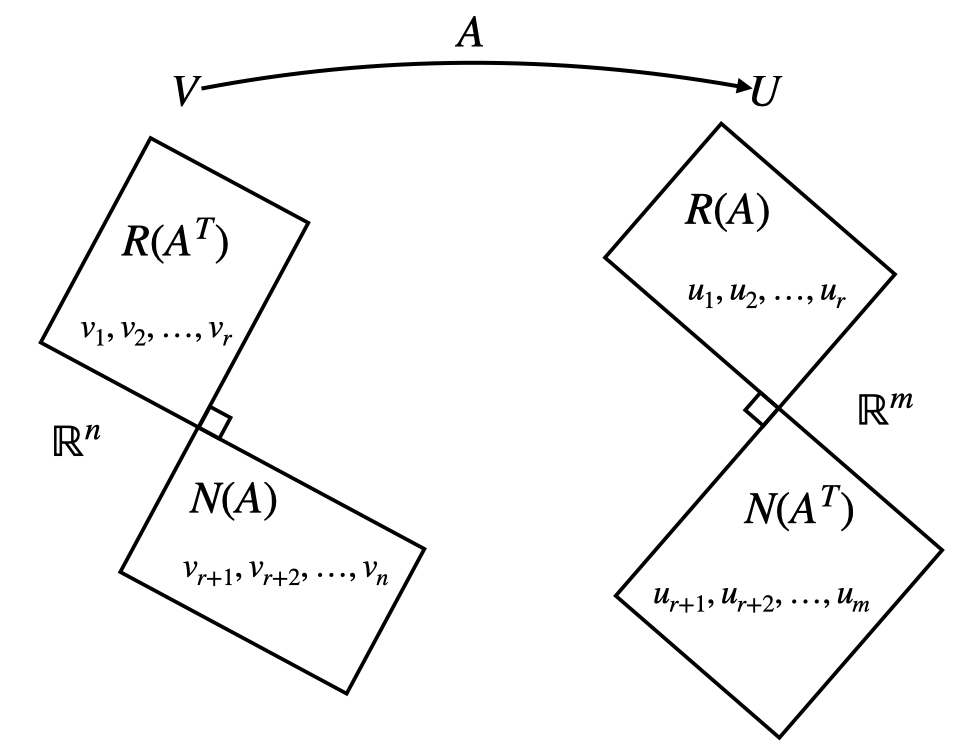
\includegraphics[width=0.5\linewidth]{figs/SVDmap.png}
\end{figure}
\end{remark}

\begin{theorem}[秩 $k$ 最佳逼近]
设 $A=U\Sigma V^H$,定义 $A_k$ 为:
\[
    A_k=\sum_{i=1}^k\sigma_iu_iv_i^H,\quad k<r
\]
则:
\begin{align*}
    &\min_{\text{rank}(B)=k}\Vert A-B\Vert_1=\Vert A-A_k\Vert_1=\sigma_{k+1}\\
    &\min_{\text{rank}(B)=k}\Vert A-B\Vert_F^2=\Vert A-A_k\Vert_F^2=\sigma_{k+1}^2+\cdots\sigma_{r}^2
\end{align*}
\end{theorem}

\begin{theorem}
设 $A=U\Sigma V^H$,则:
\begin{gather*}
    N(A)=\text{span}\{v_{r+1},v_{r+2},\ldots,v_{n}\}\\
    R(A)=\text{span}\{u_1,u_2,\ldots,u_r\}
\end{gather*}
\end{theorem}
\begin{proof}
设
\[
    A=U\Sigma V^H=\begin{bmatrix}U_1&U_2\end{bmatrix}\begin{bmatrix}\Sigma_r&O\\O&O\end{bmatrix}\begin{bmatrix}V_1^H\\V_2^H\end{bmatrix}=U_1\Sigma_rV_1^H
\]
容易验证:
\[
    U_1\Sigma_rV_1^Hx=0\iff V_1^Hx=0
\]
(1).
\begin{align*}
    N(A)&=\{x\mid Ax=0\}=\{x\mid U_1\Sigma V_1^Hx=0\}\\
    &=\{x\mid V_1^Hx=0\}=N(V_1^H)=R^{\perp}(V_1)\\
    &=R(V_2)=\text{span}\{v_{r+1},\ldots,v_n\}
\end{align*}
(2).
\begin{align*}
    &R(A)=\{y\mid y=Ax\}=\{y\mid y=U_1(\Sigma V_1^Hx)\}\subset\{y\mid y=U_1z\}=R(U_1)\\
    &R(U_1)=\{y\mid y=U_1z\}=\{y\mid y=A(V_1\Sigma_1^{-1}z)\}\subset\{y\mid y=Ax\}=R(A)\\
    \implies&R(A)=R(U_1)=\text{span}\{u_1,u_2,\ldots,u_r\}
\end{align*}
\end{proof}

\begin{theorem}[正规矩阵的奇异值分解]
设 $A$ 是正规矩阵(即 $A^HA=AA^H$),则 $A$ 酉相似于对角矩阵,即存在酉矩阵 $U$ 使得:
\[
    A=U\begin{bmatrix}
    \lambda_1&&&&&\\
    &\ddots&&&&\\
    &&\lambda_r&&&\\
    &&&0&&\\
    &&&&\ddots&\\
    &&&&&0\\
    \end{bmatrix}U^H
\]
其中 $\lambda_i$ 是 $A$ 的特征值(注意可能为负)。那么可以构造奇异值分解如下:
\[
    A=U\underbrace{\begin{bmatrix}
    |\lambda_1|&&&&&\\
    &\ddots&&&&\\
    &&|\lambda_r|&&&\\
    &&&0&&\\
    &&&&\ddots&\\
    &&&&&0\\
    \end{bmatrix}}_{\Sigma}
    \underbrace{\begin{bmatrix}
    \lambda_1/|\lambda_1|&&&&&\\
    &\ddots&&&&\\
    &&\lambda_r/|\lambda_r|&&&\\
    &&&1&&\\
    &&&&\ddots&\\
    &&&&&1\\
    \end{bmatrix}U^H}_{V^H}
\]
\end{theorem}


\begin{definition}[正交相抵]
设有矩阵 $A_{m\times n},\,B_{m\times n}$,若存在酉矩阵 $U_{m\times m},\,V_{n\times n}$ 使得 $U^HAV=B$,则称 $A$ 与 $B$ 正交相抵。
\end{definition}

\begin{property}
正交相抵是一个等价关系,即满足自反性、对称性和传递性。
\end{property}

\begin{theorem}
若 $A$ 与 $B$ 正交相抵,则 $\sigma_A=\sigma_B$.
\end{theorem}
\begin{proof}
$B=U^HAV\implies B^HB=V^HA^HUU^HAV=V^HA^HAV\implies\lambda_{B^HB}=\lambda_{A^HA}\implies \sigma_B=\sigma_A$.
\end{proof}
